\documentclass[a4paper]{article}

\usepackage{amsmath}
\usepackage{amssymb}
\usepackage{parskip}
\usepackage{fullpage}
\usepackage{hyperref}
\usepackage{xcolor}
\usepackage{stellar}
\usepackage{chronology}
\usepackage{tikz}
\usepackage{fancybox}
\usepackage{makecell}
\usepackage{bettelini}
\usetikzlibrary{cd}
\hypersetup{
    colorlinks=true,
    linkcolor=black,
    urlcolor=blue,
    pdftitle={Storia},
    pdfpagemode=FullScreen,
}

\title{Storia}
\author{Paolo Bettelini}
\date{}


\begin{document}

\maketitle
\tableofcontents
\pagebreak

% EAN 9788859300434

\section{Storia}

\sdefinition{Storiografia}{
  La \textit{storiografia} è la disciplina scientifica che si occupa di studiare la storia.
}

\section{Periodizzazione}

\sdefinition{Periodizzazione}{
  La \textit{periodizzazione} è l'operazione culturale volta a suddividere la linea temporale in vari intervalli,
  ciascuno con caratteristiche comuni.
}

Le prime periodizzazioni derivano dalle prime religioni monoteiste (Es. nascità di Gesù, calendario islamico).

Le periodizzazioni sono delle convenzioni.

\section{Fake news storiche}

% Da: Fascismo e fake news

Le fake news sono in genere effimere, ma quelle storiche sono persistenti e
pronfonde nelle persone.

\begin{itemize}
    \item Più una bugia viene ripetuta, più la si può scambiare per verità.
    \item Notizie di oggi viaggiano velocemente, è difficile bloccarle e smentirle.
    \item Comprendere il passato è un modo per comprendere il presente.
    \item Esistono fake news storiche, ancorate ad un argomento preciso.
    \item Bufale storiche vanno contrastate perché falsificano il passato (così come il ricordo e la memoria).
    \item Bufale storiche nascono da osservazioni o testimonianze inesatte, che poi si diffondono in una società pronta ad accoglierle.
    \item Bufale storiche servono ad alimentare emozioni e a rassicurare: credere in un passato positivo può portare la speranza e rischia di creare una prospettiva a cui tendere.
\end{itemize}

Effetti di scardinare le bufale:

\begin{itemize}
    \item Corregere le informazioni sul passato.
    \item Distruggere sicurezze, e ciò può creare incomunicabilità.
    \item Permette di limitare l'ambito di diffusione di queste notizie, che mistificano la memoria e la percezione del presente.
\end{itemize}

\pagebreak

\section{Linea temporale}

\begin{chronology}[250]{-1251}{2010}{\textwidth}
    \event{-1250}{Caduta di Troia}
    \event{-753}{Romolo Re di Roma}
    \event{1}{Nascita di Gesù}
    \event{622}{Egira}
    \event{800}{Carlo Magno Imperatore}
    % rinascimento
    %\event[1450]{1700}{Rinascimento}
    \event{1517}{Riforma protestante}
    % illuminismo
    \event{1789}{Rivoluzione francese}
    % romanticismo
    \event{1922}{Marcia su Roma}
\end{chronology}

\begin{chronology}*[500]{-3000}{2010}{\textwidth}
    \event{476}{Crollo Impero Romano d'Occidente}
    \event{1453}{Crollo Impero Romano d'Oriente}
    \event[-3000]{476}{Età antica}
    \event[476]{1492}{Medioevo}
    \event[1492]{1789}{Età moderna}
    \event[1789]{2010}{Età contemporanea}
\end{chronology}

% preistoria - fino a -3000

\section{Fonti}

Le fonti possono essere distinti in
\begin{itemize}
    \item \textbf{Fonti materiali:} oggetti e i reperti storici.
    \item \textbf{Fonti scritte:} scritto su carta o altri materiali storici.
    \item \textbf{Fonti figurate o iconografiche:} immagini che rappresentano eventi o scene del passato.
    \item \textbf{Fonti orali:} racconti delle persone presenti a un avvenimento.
\end{itemize}

% volontarie e involontarie, dirette indirette

\pagebreak

\section{Antico Regime}

\sdefinition{Antico Regime}{
    Una società dominata dalla disuguaglianza e dall'ingiustizia.
    Antico regime è il termine con il quale gli storici indicano l'insieme delle istituzioni
    politiche, giuridiche, economiche e sociali caratteristiche di gran parte dell'Europa tra 16°
    e 18° secolo. L'espressione ancien régime ("antico regime") fu introdotta dai rivoluzionari
    francesi del 1789 per contrapporre il vecchio regime prerivoluzionario al nuovo regime da
    loro creato in Francia con la Rivoluzione francese.
}

L'Antico regime era un tipo di società caratterizzata:
\begin{itemize}
    \item dall'autorità di un sovrano assoluto alleato con un una Chiesa
        intollerante;
    \item dal diritto fondato sulle disuguaglianze di nascita, che non
        riconosceva il valore del merito e della competenza;
    \item da un ordinamento oppressivo che imponeva ai contadini le
        servitù personali e che in generale schiacciava i sudditi sotto il
        peso delle tasse.
\end{itemize}

L'antico regime è difficile da periodizzare perché è composto da diverse
componenti di diverse epoche, anche di milleni di anni, ancora rigorosamente in vigore.

\subsection{Monarchia}

\sdefinition{Monarchia}{
    Forma di governo in cui i supremi poteri dello stato sono
    accentrati in una sola persona (re, sovrano, monarca), la cui carica non è elettiva e che può
    essere anche affiancata da altre istituzioni: m. \textit{Ereditaria}, \textit{non ereditaria}; m. \textit{Assoluta}, in
    cui il supremo governo statale è concentrato nel monarca; m. \textit{Limitata} o \textit{costituzionale},
    quando, accanto al monarca, vi sono altre istituzioni sovrane, quali il parlamento e il
    governo, che ne controllino il potere in base a una costituzione: si distingue
    la m. \textit{Costituzionale parlamentare} dalla m. \textit{Costituzionale pura} secondo che sia o no in
    vigore il principio parlamentare, ossia della necessità di un rapporto di fiducia fra
    esecutivo e legislativo.
}

Un uomo detenie quindi la sovranità, affidatagli generalmente da una divinità
per guidare il popolo verso la prosperità (legittimazione divina del potere).
La carica è ereditaria e a vita.
Nelle monarchie assolute il potete è indivisibile, è tutto nelle mani
della medesima persona.

\subsection{Repubblica}

\sdefinition{Repubblica}{
    Con riferimento all'età classica, al
    medioevo e alla prima età moderna, ogni stato non retto da un monarca o da un
    dittatore: la R. romana o di Roma, dal 509 al 31 a. C.; le r. oligarchiche della Grecia; le
    R. marinare italiane; la R. di Cromwell in Inghilterra (metà del sec. 17°), ecc. 
}

Una parte dei cittadini detiene la sovranità, che viene esercitata entro i limiti stabiliti dalle leggi.
Vi è una presenza di una pluralità di istituzioni.
La carica pubblica non è ereditaria e generalmente limitata nel tempo.\\
\textbf{\color{red}nota:} una repubblica non è necessariamente democratica.

\subsection{Impero}

\sdefinition{Impero}{
    Per impero si intende un organismo politico costituito da diversi paesi, popolazioni e Stati
collocati anche in zone non contigue, in molti casi caratterizzato dalla presenza di razze
diverse e culture e lingue non omogenee, ma sempre dotato di un centro politico e di un
nucleo nazionale dominante che esercita sull'insieme il comando e il potere supremo.
Nell'antichità e nel Medioevo a capo degli imperi vi erano i monarchi, mentre in età
moderna e contemporanea imperi sono state anche alcune repubbliche.[…]
Il maggiore e più durevole impero del mondo antico sorto in Occidente fu quello romano,
le cui origini vanno ricondotte all'opera dell'imperatore Augusto a partire dal 27 a.C.: egli
riordinò i grandi territori già conquistati da \href{http://www.treccani.it/enciclopedia/roma_(Enciclopedia_dei_ragazzi)/}{Roma} in età repubblicana, territori che
sarebbero stati ulteriormente accresciuti dai suoi successori in Europa, Asia e Africa. I
fondamenti della politica imperiale furono la superiorità militare dei Romani, una
crescente uniformità amministrativa, la diffusione della cultura greco-latina come cultura
egemone, l'allargamento della cittadinanza.\\
Data la sua estensione, l'Impero venne diviso tra il 3° e il 4° secolo in una parte occidentale
e in una parte orientale. Nel 4° secolo l'Impero divenne ufficialmente cristiano
e \href{http://www.treccani.it/enciclopedia/costantino-i-il-grande_(Enciclopedia_dei_ragazzi)/}{Costantino} spostò la capitale principale da Roma a Costantinopoli. Nel 476 l'Impero
d'Occidente crollò in seguito alle invasioni barbariche, mentre quello d'Oriente, l'\href{http://www.treccani.it/enciclopedia/impero-bizantino_(Enciclopedia_dei_ragazzi)/}{Impero bizantino},
sopravvisse fino al 1453, quando venne definitivamente abbattuto dai Turchi
ottomani.
}

\begin{itemize}
    \item Generalmente comprende vasti territori e popoli diversi, soggetti ad un'unica autorità che garantisce l'equilibrio tra le varie componenti territoriali ed etniche;
    \item sono possibili modalità di nomina diverse per l'imperatore: elezione, designazione, ereditarietà;
    \item un impero si fonda su un'ideologia a carattere universale, ovvero ha l'ambizione di costruire l'unica civiltà esistente (o comunque una civiltà superiore).
\end{itemize}

\subsection{Monarchia feudale}

\sdefinition{Feudo}{
    Grossa proprietà terriera
}

\sdefinition{Monarchia feudale}{
    Stato di proprietari, legati da un rapporto personale di subordinazione verso il sovrano che aveva donato loro la terra, e, con la terra, l'autorità.
}

In una monarchia feudale il potere del sovrano è limitato:
\begin{itemize}
    \item Non possiede una forza militare (diretta). La forza militare è quella dei feudatari che fanno giuramento verso il re;
    \item ha un potere fiscale ridotto;
    \item l'amministrazione del terrotorio e della giustizai è delegata ai signori, nobili feudatari, vassalli del re;
    \item il clero (la Chiesa) amministra le proprie terre;
    \item i comuni con status particolari (non sono sotto diretto potete del sovrano).
\end{itemize}

\sdefinition{Stato}{
    Entità giuridica dotata del monopolio amministrativo,
    giudiziario, politico e coercitivo in un determinato
    territorio, coeso e munito di precise frontiere.
}

Lo stato è quindi un territorio con dei cittadini ed un governo.

Lo stato può essere:
\begin{itemize}
    \item Autoritario (Es. Cina, Corea del Nord)
    \item Liberale/Democratico (Es. Svizzera)
    \item Unitario/Centralistico (Es. Italia, Monarchia che centra il potere)
    \item Federale (Es. Svizzera)
    \item Confederali (Es. ex Svizzera, Germania)
    \item Confessionale (Es. Vaticanow, Iran)
    \item Laico (non confessionale)
    \item Socialista (Es. Cina, Cuba, Corea del Nord)
    \item Capitalista
\end{itemize}

\sdefinition{Stato Moderno}{
    Lo \textit{stato moderno} è sorto in Europa
    tra il 15° e il 16° secolo, trovando la sua espressione dominante nella monarchia assoluta, che
    a partire dalle grandi monarchie nazionali di Spagna, Inghilterra e Francia pose gradualmente
    fine al particolarismo di matrice feudale o quanto meno lo ridusse fortemente ponendolo
    sotto il proprio controllo.
}

I suoi membri - individui e organismi collettivi - sono sottomessi unicamente alla legge,
garanzia dei diritti statuiti e sottoposti al controllo dell'ordine giudiziario.

Il primo tipo di stato è stato lo stato moderno, che poi si è trasformato in stato liberale democratico
nei tempi moderni.
Vi sono principalmente tre fattori che hanno procurato il passaggio da monarchia feudale a stato moderno:

\begin{itemize}
    \item
    Il passaggio dal Medioevo al Rinascimento ha visto un profondo cambiamento nell'assolutismo, che non era più solo teorico ma divenne effettivo nel Cinquecento e Seicento. Questo cambiamento è attribuibile principalmente alla nuova struttura dello Stato, in particolare all'istituzione di eserciti permanenti che garantivano il potere del re. Questi eserciti, sia sotto forma di guarnigioni fisse che di truppe mobili, erano ora composti da fanterie mercenarie dipendenti solo dal re e non più dalla feudalità. La fanteria, diventata la principale forza militare, consentiva al sovrano di esercitare una politica estera più ampia.
    \item
    Inoltre, si è assistito a un cambiamento nella politica estera con l'organizzazione della prima diplomazia permanente, contrariamente al Medioevo in cui le relazioni internazionali erano meno strutturate. Questo cambiamento ha portato all'idea di equilibrio di potere tra gli Stati europei.
    \item
    Oltre all'esercito e alla diplomazia, la burocrazia statale è emersa come elemento chiave, con una crescente potenza degli "ufficiali"/funzionari del sovrano. In questo periodo, lo Stato si è concentrato attorno al potere sovrano e alla gerarchia degli ufficiali, piuttosto che sugli "ordini" della nazione o gli Stati generali.
    Vendita della cariche.
\end{itemize}

Questi processi mirano i ridurre il potere dei feudali ed aumentare quello del sovrano.

Nel 1685 Luigi XIV comanda tutti gli Ugonotti di convertirsi al cristianesimo creando
un'uniformità religiosa.

Il Re diventato lo Stato sotto tutti gli effetti.

\subsection{La Società dell'Antico Regine}

\begin{center}
    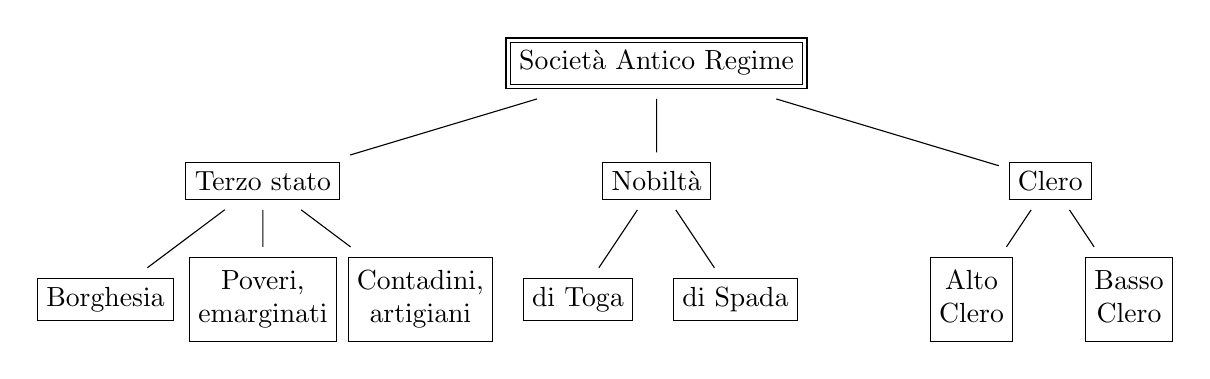
\begin{tikzpicture}[
        level 1/.style = {sibling distance = 5cm},
        level 2/.style = {sibling distance = 2cm}
    ]
    \node {\doublebox{Società Antico Regime}}
        child {
            node {\fbox{Terzo stato}}
            child {
                node {\fbox{Borghesia}}
            }
            child {
                node {\fbox{\makecell[c]{Poveri, \\ emarginati}}}
            }
            child {
                node {\fbox{\makecell[c]{Contadini, \\ artigiani}}}
            }
        }
        child {
            node {\fbox{Nobiltà}}
            child {
                node {\fbox{di Toga}}
            }
            child {
                node {\fbox{di Spada}}
            }
        }
        child {
            node {\fbox{Clero}}
            child {
                node {\fbox{\makecell[c]{Alto \\ Clero}}}
            }
            child {
                node {\fbox{\makecell[c]{Basso \\ Clero}}}
            }
        };
    \end{tikzpicture}
\end{center}

Non si può accedere al clero per nascita.
Le tasse appartengono unicamente a quelli appartenenti al terzo stato.
Non vi è libertà di pensiero, culto o parola.

Questo tipo di società è divisa per discendenza eccetto per il Clero.
Il primo genito di una famiglia nobiliare eredita spesso le varie terre, mentre il secondo genito
andrà a fare parte dell'Alto Clero, mentre il Basso Clero è principalmente occupato dalla Borghesia.

\subsection{Fallimento dell'accentramento monarchico in Inghilterra}

Carlo I Stuart fu il primo sovrano decapitato dal popolo.
Il parlamento in inghilterra non si fa scavalcare, e i sovrani, a differenza di quelli francesi,
non riescono così tanto a centralizzare il potere.
Il parlamento si ribella e obbliga i nuovi sovrani di firmare il "Bill of rights".

\sdefinition{Bill of Rights}{
    Il parlamento impone (non chiede) al sovrano di essere riconosciuto.
}

\begin{itemize}
    \item Il potere limtiato dal re;
    \item un parlamento rappresentativo dotato del monopolio legislativo;
    \item sistenza giudiziario a garanzia dell'integrità delle persone e di alcuni diritti indivuduali
\end{itemize}

Alcuni elementi per essere uno Stato moderno sono assenti, il potere non è infatti centralizzato.
Tuttavia, è uno Stato Moderno perché riconosce i diritti individuali nei confronti del potere dello Stato.
Seppur limitato, il otere del sovrano viene esercitato in modo uniforme su tutti i sudditi e su tutto il territorio.

Il potere statuale non è più concentrato, bensì ripartito tra figure diverse:
\begin{itemize}
    \item il re possiede il potere esecutivo;
    \item il parlamento ha potere legislativo;
    \item giudici hanno potere giudiziario.
\end{itemize}

% TODO stato liberale rappresentativo e le costituzioni
% TODO differenza fra monarchia costituzionale e parlamentare

\subsection{Illuminismo}

\sdefinition{Illuminismo}{
    L'\textit{illuminismo} è una corrente di pensieri anche nominata l'età dei lumi.
    La luce alla quale si fa riferimento è in diretta contrapposizione
    al medioevo e diverse concezioni dell'Antico Regime, ossia, all'ignoranza.
}

L'illuminismo è caratterizzato dall'autonomia dell'individuo e uso della ragione.
Un movimento cosmopolita (La Natura, Il Cosmo sono gli stessi ovunque si metta piedei. Perciò essi
potevano vivere allo stesso modo in accordo con la natura ovunque. Essi non erano a casa in una città
o in un'altra, ma nella natura, nel Cosmo. Si chiamavano infatti cittadini del Cosmo: cosmopoliti).
Inoltre, era caratterizato dalla tolleratanza; libertà di coscienza e di opinione.

% TODO def intolleranza. di alberto pincherie Encliclopedia italiana 1933
Possiamo cominciare a parlare di tolleranza quando vi sono motleplici religioni o teismi che sostengono di possedere la verità assoluta, le quali vanno in conflitto diretto con le altre.
\sdefinition{Giusnaturalismo}{
    Il \textit{giusnaturalismo} è corrente filosofica giuridica, fondata su due principi:
    \begin{itemize}
        \item esiste un diritto naturale (conforme cioè alla natura dell'uomo e quindi intrinsecamente corretto);
        \item è superiore al diritto positivo (diritto prodotto dagli uomini).
    \end{itemize}
}

Esistono norme di diritto naturale che hanno per oggetto la tutela della vita, della libertà e della proprietà.

Nasce l'idea di avere un governo composto da 3 organi \textbf{separati}
e \textbf{indipendenti} in maniera take che essi si bilancino e si frenino a vicenda.

\subsection{Voltaire}

\sdefinition{Dispotismo illuminato}{
    Il \text{dispotismo illuminato} è il governo assolutista di un monarca o despota illuminato.
}

Voltaire porta avanti il concetto di dispotismo assolutismo ma illuminato (intellettuali illuministri, consiglieri).
Il popolo va governato usando la ragione.

\subsection{Rousseau}

Rousseau, mediante il \textit{Contratto Sociale} (1762),
cercare di ridefinire il modo di vivere definendo una \textit{repubblica democratica}.
Questo repubblica è di uguaglianza, tutti hanno gli stessi diritti degli altri.

Piuttosto che prioritizzare l'individuo, si prioritizza collettivamente una meta comune
che viene seguita con la \textit{volontà generale}.

\begin{itemize}
    \item Gli uomini devono esercitare la libertà di fare le leggi (democrazia diretta);
    \item nel contratto sociale Rousseau ipotizza un patto in cui gli uomini non perdono mai la libertà nè la sovranità: questo patto è chiamato \textit{contratto sociale} e fonda la democrazia.
    \item senza il patto non c'è sovranità legittima;
    \item il patto fa entrare gli individui in una società politica: gli uomini si uniscono e nasce la volontà collettiva;
    \item gli uomini non si assoggettano, non cedono la sovranità a qualcuno, ma a sè stessi, ad un'assemblea di cittadini;
    \item nasce un io collettivo, comunità politica, nata in seguito ad un contratto.
\end{itemize}

\subsection{La Dichiarazione di Indipendenza degli Stati Uniti (1776)}

Il documento enuncia i principi dei diritti dell'uomo e della legittimità della rivoluzione,
principi derivanti dall'illuminismo.
Questi principi giustificano la rivoluzione e le colonie hanno quindi il diritto di
diventare indipendenti dalla Gran Bretagna.

% TODO winner takes all
% la corte suprema si occupa di verificare che le leggi siano costituzionali
% può invalidare le leggi se rischia di essere anti costituzionale
% check and balance | controlla / veto

\subsection{Le rivoluzioni americana e francese}

\begin{itemize}
    \item Una costituzione che limita il potere dello Stato con la divisione dei poteri.
    \item Una democrazia rappresentativa.
    \item Una potere repubblicano e/o monarchico costituzionale.
    \item Il riconoscimento dei diritti individuali e naturali dell'individuo.
\end{itemize}

Tutti sono uguali davanti alla legge, a differenza della società dell'Antico Regime,
dove vi erano dei privilegi.

\subsection{La Dichiarazione dei diritti dell'uomo e del cittadino}

\begin{enumerate}
    \item Gli uomini nascono e rimangono liberi e uguali nei diritti. Le distinzioni sociali
    non possono essere fondate che sull'utilità comune.
    \item Il fine di ogni associazione politica è la conservazione dei diritti naturali ed
    imprescrittibili dell'uomo. Questi diritti sono la libertà, la proprietà, la sicurezza e la
    resistenza all'oppressione.
    \item Il principio di ogni sovranità     risiede essenzialmente nella \textit{Nazione}.
    Nessun corpo o individuo può esercitare un'autorità che non emani espressamente da essa.
    \item La libertà consiste nel poter fare tutto ciò che non nuoce ad altri: così, l'esercizio
    dei diritti naturali di ciascun uomo ha come limiti solo quelli che assicurano agli altri
    membri della società il godimento di questi stessi diritti. Questi limiti possono essere
    determinati solo dalla Legge.
    \item  La legge ha il diritto di vietare solo le azioni nocive alla società. Tutto ciò che non
    è vietato dalla Legge non può essere impedito, e nessuno può essere costretto a fare ciò
    che essa non ordina.
    \item La Legge è l'espressione della volontà generale. Tutti i cittadini hanno il diritto di
    concorrere, personalmente o mediante i loro rappresentanti, alla sua formazione. Essa
    deve essere uguale per tutti, sia che protegga, sia che punisca. Tutti i cittadini essendo
    uguali ai suoi occhi sono ugualmente ammissibili a tutte le dignità, posti e impieghi
    pubblici secondo la loro capacità, e senza altra distinzione che quella delle loro virtù e
    dei loro talenti.
    \item Nessun uomo può esser accusato, arrestato o detenuto se non nei casi determinati
    dalla Legge, e secondo le forme da essa prescritte. Quelli che procurano, emettono,
    eseguono o fanno eseguire degli ordini arbitrari, devono essere puniti; ma ogni cittadino
    citato o tratto in arresto, in virtù della Legge, deve obbedire immediatamente;
    opponendo resistenza si rende colpevole.
    \item La Legge deve stabilire solo pene strettamente ed evidentemente necessarie e
    nessuno può essere punito se non in virtù di una legge stabilita e promulgata
    anteriormente al delitto, e legalmente applicata.
    \item Presumendosi innocente ogni uomo sino a quando non sia stato dichiarato
    colpevole, se si ritiene indispensabile arrestarlo, ogni rigore non necessario per
    assicurarsi della sua persona deve essere severamente represso dalla Legge.
    \item Nessuno deve essere molestato per le sue opinioni anche religiose, purché la
    manifestazione di esse non turbi l'ordine pubblico stabilito dalla Legge.
    \item La libera comunicazione dei pensieri e delle opinioni è uno dei diritti più preziosi
    dell'uomo; ogni cittadino può dunque parlare, scrivere, stampare liberamente, salvo
    rispondere all'abuso di questa libertà nei casi determinati dalla Legge.
    \item La garanzia dei diritti dell'uomo e del cittadino ha bisogno di una forza pubblica;
    questa forza è dunque istituita per il vantaggio di tutti e non per l'utilità particolare di
    coloro ai quali essa è affidata.
    \item Per il mantenimento della forza pubblica, e per le spese d'amministrazione, è
    indispensabile un contributo comune: esso deve essere ugualmente ripartito fra tutti i
    cittadini, in ragione delle loro sostanze.
    \item Tutti i cittadini hanno il diritto di constatare, da loro stessi o mediante i loro
    rappresentanti, la necessità del contributo pubblico, di approvarlo liberamente, di
    controllarne l'impiego e di determinarne la quantità, la ripartizione, la riscossione e la
    durata.
    \item La società ha il diritto di chieder conto a ogni agente pubblico della sua
    amministrazione
    \item Ogni società in cui la garanzia dei diritti non è assicurata, né la separazione dei
    poteri determinata, non ha costituzione.
    \item La proprietà essendo un diritto inviolabile e sacro, nessuno può esserne privato,
    salvo quando la necessità pubblica, legalmente constatata, lo esiga in maniera evidente,
    e previa una giusta indennità.
\end{enumerate}

Il terzo articolo elimina ciò che è il potete divino all'interno della sovranità,
e lo rimpiazza con solo ed unicamente il volere della nazione stessa.

Il sesto articolo rompe la possibilità di acquistare o ereditare cariche di posizione.

% Napoleone permette di esportare questi principi all'estero, fino in Svizzera.

\section{L'Ottocento}

\sdefinition{Restaurazione}{
    Periodo della storia europea che va dalla fine del regime napoleonico
    all'abdicazione del re di Francia Carlo X di Borbone.
}

\sdefinition{Santa Alleanza}{
    La \textit{Santa alleanza} è stata una coalizione tra le grandi potenze monarchiche della Russia, dell'Austria e della Prussia.
    La Santa Alleanza fu creata dopo la sconfitta di Napoleone.
}

\subsection{Liberalismo}

Principalmente possiamo distinguere il \textit{movimento liberale} (non ancora \textbf{partito})
e il \textit{movimento conservatore}.

Il liberalismo è caratterizzato dalle seguenti proprietà:
\begin{itemize}
    \item Fiducia nell'individuo.
    \item Libertà individuo di fronte allo Stato.
    \item Libertà dell'individuo devono essere garantite.
    \item Aspirazioni della ricca borghesia.
    \item Libertà e uguaglianza \(\rightarrow\) entrano in conflitto.
    \item Movimento democratico-liberale \(\rightarrow\) uguaglianza.
    \item Sovranità popolare \(\rightarrow\) individuo partecipa alle attività dello Stato.
\end{itemize}

Il movimento liberale ha origini in realtà nel 1700 perché si oppone
all'assolutismo monarchico, assolutismo che tornerà nel 1800 con la restaurazione.
Ha le sue radici nelle idee dell'illuminismo e nei principi di libertà individuale e di autodeterminazione.

Viene rimpiazzata la monarchia costituzionale con il parlamento eletto (suffragio censitario)
\(\rightarrow\) sovranità nazionale.
Il potere dello Stato deve essere limitato e favorire la libertà d'azione.

\subsection{Liberalismo moderato o conversatore}

\textbf{Libertà da:}
\begin{itemize}
    \item \textbf{Libertà dallo Stato:} Questo concetto è legato alla cosiddetta libertà negativa, che si riferisce alla protezione dell'individuo
        dall'interferenza o coercizione dello Stato o di altri individui.
        Nel contesto storico menzionato nel documento, questo concetto è particolarmente
        rilevante durante il secolo XVIII, un periodo in cui si iniziava
        a chiedere un minor intervento dello Stato nella vita delle persone.
\end{itemize}

\textbf{Libertà di:}
\begin{itemize}
    % di partecipare alla vita politica
    \item \textbf{Libertà di parola, riunione, associazione:} Questi sono diritti fondamentali che il liberalismo sostiene debbano essere protetti da qualsiasi forma di oppressione o limitazione.
    \item \textbf{Libertà di stampa, culto, attività economica:} Allo stesso modo, queste libertà sono viste come essenziali per il pieno sviluppo e la realizzazione dell'individuo.
    \item \textbf{Diritto inviolabile della proprietà:} Questo è un pilastro fondamentale del pensiero liberale, che vede la proprietà privata come un diritto sacro e inviolabile.
\end{itemize}

Il ceto sociale di riferimento è la borghesia, per cui il sistema è verticista e censitario (solo chi
ha le capacità, il tempo ed è proprietario o contribuisce alla ricchezza dello Stato può governare
ed è in grado di farlo).
Si mira a favorire in primo luogo lo sviluppo economico e di riflesso anche la stabilità sociale.

\begin{itemize}
    \item Più lo stato è limitato, più l'uomo è libero di agire (in contrapposizione con l'assolutismo).
    \item Libertà sì, ma con moderazione, libertà di voto ma non per tutti (solo possedenti). Realizzazione graduale dell'assetto del liberalismo, possono scendere a compromessi con l'antico regime.
\end{itemize}

\subsection{Liberalismo radicale o democratico}

In generale si riprendono i prinipi del liberlismo, ma in modo più radicale.
Invece ad una monarchia parlamentare, preferiscono una repubblica con un sistema rappresentativo (suffragio universale).

\begin{itemize}
    \item L'uomo è tanto più libero se può esercitare le prorpie libertà, se non è limitato o escluso dalla povertà o dalla malattia, chi lo è non ha i mezzi per poter godere delle proprie libertà.
    \item Trasformazione rapida della società, cambiamento deciso; volontà di stravolgere la società di antico regime. Vogliono coinvolgere tutta la popolazione (democratici): referendum, suffragio universale.
\end{itemize}

Il liberalismo radicale presta maggiore attenzione ai ceti popolari e mira a coniugare sviluppo
economico e stabilità sociale. La corrente radicale, che promuove in modo particolare
l'uguaglianza economica e sociale si avvicina al pensiero socialista (senza però l'abolizione della
proprietà privata)

\subsection{Pensiero conservatore}

\sdefinition{Conservatorismo}{
    Con \textit{conservatorismo} si intende l'insieme delle ideologie che, variamente, si oppongono al progresso. Il
concetto di conservatorismo appartiene esclusivamente al lessico politico moderno.
}

Il partito conservatore fra il '700 e '800 si opponeva all'illuminismo e a tutto ciò che portava la Rivoluzione Francese.
Il pensiero conservatore è l'antitesi del liberalismo.

Si oppone originariamente al concetto di eguaglianza fra gli umani. Secondo loro, le differenze fra gli uomi sono naturali.

\pagebreak

\subsection{Schema riassuntivo}

\begin{enumerate}
    \item \textbf{Risoluzionari}: Cambiamento radicale forzato uso della violenza.
    \item \textbf{Progressisti}: Cambiamento graduale tramite riforme.
    \item \textbf{Conservatori}: Rispetto della tradizione, mutare il presente nel rispetto della tradizionare.
    \item \textbf{Reazionari}: Vogliono ritornare ad un regime precedente.
\end{enumerate}

\textbf{Conservatori:}
\begin{itemize}
    \item Monarchia assoluta.
    \item Rafforzamento delle gerarchie di potere (clero e nobiltà).
    \item Difesa della tradizione.
    \item Potere per diritto divino, nessuna rappresentanza popolare.
\end{itemize}

\textbf{Liberali:}
\begin{itemize}
    \item Monarchia costituzionale.
    \item Rispetto dell'autonomia dell'individuo e della ragione.
    \item Idea di progresso
    \item Potere delle èlite borghesi, che devono essere rappresentate.
\end{itemize}

\subsection{Socialismo}

A partire dagli anni Venti dell'Ottocento, i termini socialismo e socialisti vennero usati per
definire l'atteggiamento critico assunto, da numerosi intellettuali, nei confronti dei
problemi provocati dal processo di industrializzazione. Più esattamente, le due espressioni
appena citate furono impiegate per indicare la posizione di coloro che, come rimedio alle
drammatiche condizioni degli operai e alla diseguaglianza sociale, proponevano la
soppressione della proprietà privata e la tutela delle classi dei lavoratori.

\begin{enumerate}
    \item Con la rivoluzione industriale;
    \item muta in modo drastico la vita di milioni di essere umani;
    \item radicale cambiamento nel sistema di produzione;
    \item massiccio impiego di donne e bembini;
    \item sorgono, nelle città, quartieri operai privi di servizi elementari;
    \item trasformazione del mondo agricolo a quello industriale, con conseguenze mutamento della società e l'emergere di nuove classi sociali (borghesia / proletariato).
\end{enumerate}

I primi sindacati furono le \textit{Trade Unions} in Inghilterra, occupandosi si salvaguardare il proletariato.

\sdefinition{Socialismo}{
    Il socialismo, a partire dagli anni Venti dell'Ottocento, rappresentava una reazione critica all'industrializzazione, sostenendo la soppressione della proprietà privata e la protezione dei lavoratori come rimedio alle condizioni drammatiche degli operai e alla disuguaglianza sociale.
}

\textbf{Socialismo utopico}: Le figure chiave del socialismo utopico includono Charles Fourier e Robert Owen.
Questi pensatori immaginavano comunità ideali basate sulla cooperazione e l'uguaglianza,
ma spesso mancavano di un piano dettagliato per attuare queste visioni nella pratica.
Il socialismo utopico è stato successivamente superato dall'approccio più scientifico
ed economico del socialismo marxista.

Esistono quindi altri tipologie di socialismo, come quello \textbf{scientifico}.
Secondo i socialisti, specialmente quelli scientifici, abolire la proprietà privata
potrebbe portare a qualcosa di nuovo e rinnovato.

Le idee possono essere riassunte con i seguenti punti:
\begin{enumerate}
    \item Il socialismo (e successivamente comunismo) va applicato gradualmente. In primis, quando il capitalismo entrerà in contradizione con sè stesso.
    Questa contraddizione deriveré dallo scontro fra borghesia e proletariato.
    \item Lotta di classe, ossia l'idea cje la società umana sia passata attraverso 4 fasi
    (comunità primitive, regime di schiavitù, società feudale, società borghese).
    Per cui l'intera società è costituita da uno scontro fra gli oppressori ed oppressi.
    \item Tutto, fra cui i pensieri, scaturisca dal materialismo e dai bisogni umani.
    Divisione fra \textbf{struttura} (modi di produzione della ricchezza)
    e \textbf{sovrastruttura} (politica, arte, religione, etc).
    Dai modi di produrre ricchezza, si sviluppana la società con le sue idee.
    Se non ci sono classi sociali non ci possono essere lotte di classe.
\end{enumerate}

\begin{figure}[h]
    \centering
    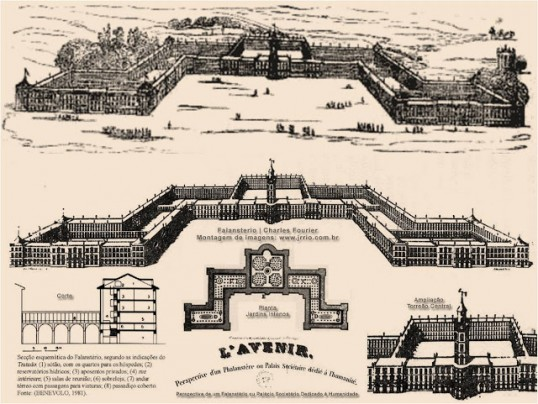
\includegraphics[width=0.75\textwidth]{./falansterio.jpg}
\end{figure}


Secono il testo di Marx, la vittoria è quando abbiamo una massima unità del proletariato.
Per ottenere il dominio sulla classe borghese è necessario accumulare ricchezza e capitale.
Questo ricchezza va ottenuta mente il lavoro salariato, il quale fonda concorrenza fra operai.
Ciò porta al progresso dell'industria ma sostiuisce l'isolamento degli operai con associazione degli operati (unione del proletariato).

Nonostante viene ritenuto che questa rivoluzione sarebbe prima o poi avvenuta, gli operai e il proletariato,
pur essendo la maggioranza, non giungono a questa meta.

Fino al 1970 circa i termini marxismo e leninismo sono praticamente sinonimi.
Rimangono comunisti tutti coloro che ritengo che la lotta di classe sia inevitabile.

\pagebreak

\subsection{Nazione, Nazinoalità, Nazionalismo}

\sdefinition{Nazione}{
    Nel medioevo, \textit{nazione} aveva un significato puramente geografico.
    Ma dagli inizi dell'Ottocento, nel clima del Romanticismo, il
    termine nazione si carica di un nuovo significato e indica una individualità storica, una
    comunità umana, un popolo che si differenzia da altri popoli sulla base delle sue
    caratteristiche: il profilo etnico o la consanguineità, il legame con un territorio, la lingua, la
    cultura, le esperienze storiche, le consuetudini che regolano la vita comune, le tradizioni
    civili e religiose.
}

Quando consideriamo un fattore etnico abbiamo il \textit{concetto naturalistico},
entre quando parliamo di stare assieme sulla base di esperienze comuni, abbiamo il \textit{concetto volontaristico}.
Quest'ultimo concetto ci dice che la nazione è un prodotto culturale.

\textbf{Renan: Cos'è una nazione (concetto volontaristico)}
\begin{itemize}
    \item Caratteristice legate alla cultura, alla storia;
    \item condivisione di cultura, modo di fare;
    \item eredità di ricordi e consenso attuale \(\rightarrow\) eredi di un patrimonio;
    \item è una scelta.
    \item Prima nasce lo Stato, poi la Nazione.
\end{itemize}

\textbf{Fichte: Cos'è una nazione (concetto naturalistico)}
\begin{itemize}
    \item Stirpe/origini/lingua/territoria;
    \item lingua \(\rightarrow\) recupero dell'identità originaria della nazione;
    \item non è una scelta.
    \item Prima nasce la Nazione, poi lo Stato.
\end{itemize}

\textbf{Concetto volontaristico:}
\begin{itemize}
    \item Sentimento di identità e spinta a stare assieme sulla base di esperienze comuni.
    \item Nazione come prodotto culturale in cui si valorizzano gli aspetti storici e ideali che connotano un popolo.
    \item Idea di poter scegliere.
    \item Concetto volontaristico, volontà di condividere principi, valori, comune sentire.
    \item Illuminismo e riv. Francese come radici culturali di questo concetto (concezione francese).
\end{itemize}

\textbf{Concetto naturalistico:}
\begin{itemize}
    \item Fattori etnici: la nazione è un fattore naturale, oggettivo, basato su elementi come l'etnia, il territorio (lingua, letteratura, tradizioni culturali).
    \item L'appartenenza nazionale di una persona è predestinata (non si può scegliere).
    \item Romanticismo e Restaurazione ne sono il contesto (concezione tedesca).
\end{itemize}

\pagebreak

\section{La Svizzera}

\subsection{Confederazione dei 13 Cantoni}

La Confederazione dei 13 Cantoni era fondamentalmente suddivisa in 3 gruppi territoriali.
\begin{itemize}
    \item Cantoni sovrani (3);
    \item 11 Alleati;
    \item paesi / Territori soggetti, (baliaggi).
\end{itemize}

Vi è una ampia autonomia delle comunità locali (Entità indipendente del Sacro Romano Impero Germanico dal 1698).
Le città sono principalmente composte da governi oligarchici, mentre verso le comunità
vi erano le landsgemeinde (assemblee) di contadini proprietari.
\sdefinition{Oligarchia}{
    Con \textit{oligarchia} si indica il governo di pochi (es. famiglia importanti, influenti).
}
La Svizzera del tempo è quindi frammentata, ma viene tenuta assieme da una Dieta.
\sdefinition{Dieta}{
    La \textit{Dieta} è un'assemblea generale di delegati dei Cantoni (e di alcuni alleati).
}

Ogni decisione doveva essere presa all'unanimità.
La Dieta dei cantoni cattolici si riuniva separatamente da quella di Protestanti.
Non c'è un esercito unitario e una vera e propria politica estera.
Inoltre, la Svizzera ha una lunga tradizione di \textit{mercenariato} che, per i cantoni più rurali,
è un importante entrata economica.
L'ultima Dieta avvenne nel 1798.
A turni, ogni cantone mandava un landfogto nei comuni per essere amministratori.

La Svizzera è quindi composta da enti separati che sono tutti collegati da una cosa ccentrale, come il patto o la Dieta.

\subsection{Confederazione e federazione}

La confederazione è un'alleanza tra Stati, mentre la federazione è un unico Stato,
anche se composto di parti (Stati o regioni) che godono di una larga autonomia.
Tra una confederazione e una federazione vi sono numerose soluzioni istituzionali intermedie.
La Svizzera è una federazione nonostante sia rimasto il nome di tradizione di confederazione.

\subsection{Club helvétique}

\sdefinition{Club helvétique}{
    Il \textit{Club helvétique} è un club di svizzeri a Parigi.
    Essi comunicano con i francesi e sostengono l'espansione delle idee derivanti dalla Rivoluzione Francese
    in Svizzera.
}

\subsection{La Repubblica elvetica (1798 - 1802)}

Dal 1798 la Svizzera passa da una confederazione ad una repubblica (una e indivisibile),
ossia un regime imposto dalla Francia.
In questa repubblica vengono aboliti i baliaggi, ma vengono definiti come \textit{unità amministrative}.

% TODO metti le due diverse costituzioni LA SVIZZERA DALLA VECCHIA CONFEDERAZIONE AL 1848

\pagebreak

Le riforme introdotte con la Repubblica sono le seguenti:
\begin{itemize}
    \item Usuaglianza dei cittadini di fronte alla legge;
    \item suffragio universale (maschile);
    \item libertà di pensiero, di stampa, di religione;
    \item libertà di domicilio e industria;
    \item viene creata la cittadinanza svizzera: le persone non sono più unicamente cittadini dei loro cantoni;
    \item divisione dei poteri secondo il principio di Montesquieu;
    \item unificazinoe dei pesi, delle misure e della moneta.
    \item soppressione delle dogane interne;
    \item obbligatorietà dell'insegnamento elementare.
\end{itemize}

La Repubblica Elvetica è tuttavia molto politicamente instavbile e termina nel 1802.

\subsection{Atto di Mediazione (1802/1803-1810)}

\begin{center}
    \begin{tikzcd}
        & \fbox{\textit{Mediazione}} & \\
        \makecell{\text{Federalisti} \\ \text{(cattolici)}} & & \makecell{\text{Repubblicani} \\ \text{(centralisti)}}
    \end{tikzcd}
\end{center}

I federalisti sono favorevoli all'autonomia cantonale, ossia ciò che c'era prima della repubblica elvetica.
I repubblicani sono invece favorevoli ad uno stato unitario, un un unico governo indivisibile e dove i cantoni non hanno automonie.
I federalisti sono quindi tradizionalisti, a differenza dei repubblicani.

\sdefinition{Atto di mediazione (1802/1803-1810)}{
    L'\textit{atto di mediazione} è stato imposto da Napoleone alla Svizzera per
    applicare una nuova Costituzione di stampo maggiormente federalistico e
    dunque con maggiori poteri attribuiti ai Cantoni.
}

Io scopo questo atto perché secondo Napoleone è quello di aiutare la Svizzera con un compromesso.
Questo atto provvede:
\begin{itemize}
    \item libertà fondamentali che vengono garantite, uguaglianza cittadini di fronte alla legge, soppressione dogane interne;
    \item scioglimento del vecchio governo centrale (repubblica);
    \item ogni cantone ha la propria costituzione e ampia autonomia;
    \item vi è un'autorità centrale (la Dieta federale, composta da 25 membri, non un parlamento).
\end{itemize}

Questa nuova costituzione porta alla Svizzera formata da 19 cantoni tutti di pari rango.
La Dieta, la quale si riunisce una volta all'anno come congresso dei delegati,
rappresenta quindi l'autorità centrale.

I compiti e capacità della Dieta:
\begin{itemize}
    \item promulgare dei decreti;
    \item dichiarare guerra;
    \item firmare e ratificare la pace;
    \item concludere alleanze e trattati commerciali.
\end{itemize}

Il potere viene suddiviso con \\
\textbf{legislativo} \(\rightarrow\) Gran Consiglio (110 deputati) \\
\textbf{esecutivo} \(\rightarrow\) Piccolo Consiglio.

\begin{figure}[h]
    \centering
    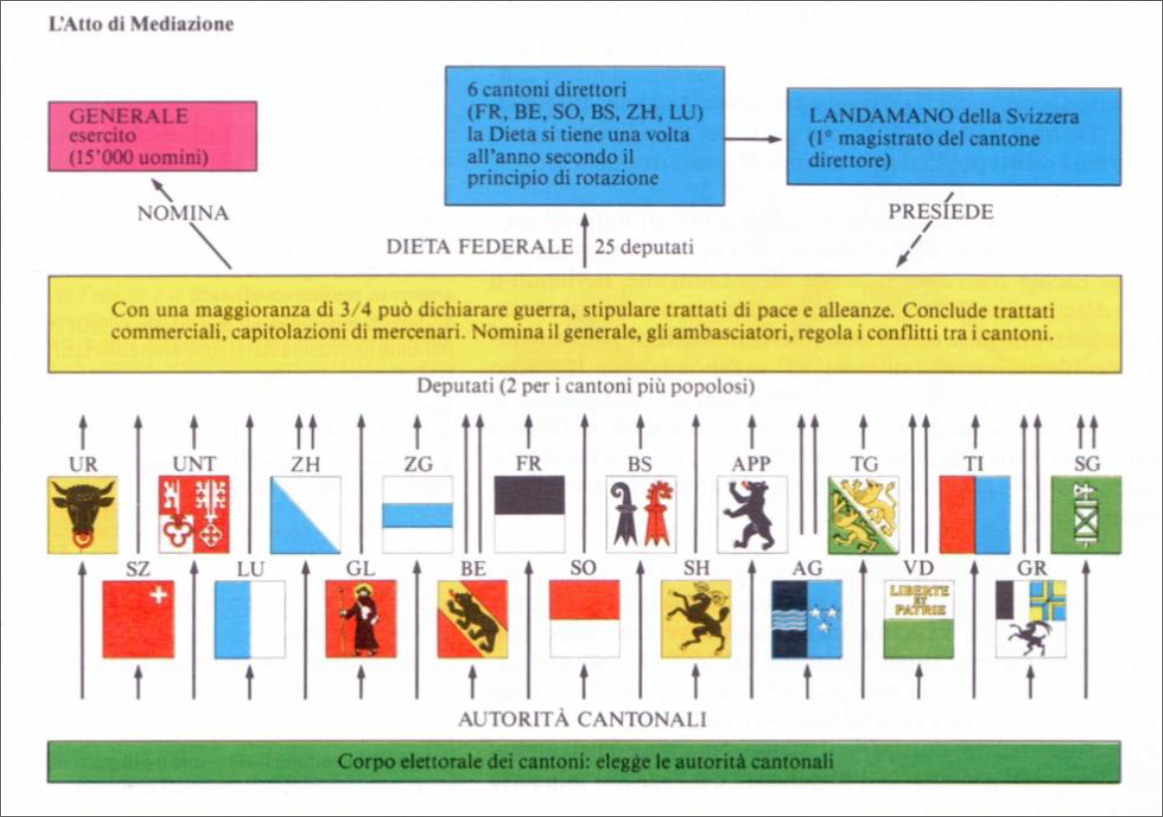
\includegraphics[width=0.75\textwidth]{./mediazione.png}
\end{figure}

\subsection{Restaurazione}

Nel 1815 le potenze europee che avevano sconfitto Napoleone (vincitrici del Congresso di Vienna)
volevano ripristinare in parte gli equilibri prerivoluzionari.
In Svizzera ciò avvenne con il Patto federale del 1815 che
accordò ai Cantoni la quasi completa autonomia amministrativa.

\sdefinition{Patto del 1815}{
    Il \textit{patto del 1815} è una costituzione che crea una confederazione elvetica di 23 cantoni.
}

Le potenze assicurarono alla Svizzera la neutralità perpetua e garantirono
l'integrità e l'inviolabilità del territorio svizzero allargato.
Esso ridisegna la cartina europa e viene riconosciuto a livello internazione la neutralità elvetica perpetua.

La Svizzera prende il nome ufficiale di Confederazione Svizzera, con 23 cantoni sovrani.
Nascono quindi istituzioni conservatrici in Svizzera.
La Dieta federale esiste ancora ma ha meno potere.
Inoltre, vi è un esercito unico per la prima volta.
Tornano tuttavia le dogane interne, ostacolando il traffico doganale, e quindi facendo
soffrire la Svizzera economicamente.
La Svizzera può stipulare una pace o dichiarare una guerra se ha una maggioranza di \(\frac{3}{4}\),
mentre per altre questioni una maggioranza semplice.

\subsection{Influenza liberale dal 1830}

Nonostante la corrente restaurativa, la Svizzera rimane
comunque aperta verso gli esuli delle altre nazioni.
Infatti, la Svizzera diventa terra d'asilo per gli esuli del liberalismo.
Questa situazione favorisce il progresso liberalista.

Dopo la rivoluzione parigina del 1830, la metà circa dei cantoni, fra i quali Berna, Zurigo,
Lucerna, Vaud, Friborgo riformarono le loro costituzioni in senso democratico,
abolirono le antiche imposizioni feudali, garantirono le libertà politiche fondamentali.

La riforma del sistema politico federale costituisce il principale pomo della discordia
tra liberali-radicali e conservatori. I primi pronti ad usare la forza per riformare il Patto
del 1815 al fine di creare uno stato con un potere centrale più forte. I secondi si
pongono come i più decisi sostenitori della sovranità cantonale. Le questioni religiose
complicano un conflitto che è essenzialmente di natura politica: i liberali radicali sono
fautori di una società laica e vedono nel cattolicesimo un ostacolo alla modernizzazione
del paese, che viene invece strenuamente difeso dai conservatori.

In seguito ai tentativi dei radicali di rovesciare con la forza il governo di Lucerna (1844-45)
i cantoni conservatori cattolici (Lucerna, Uri, Schwyz, Unterwald, Friburgo, Vallese)
costituirono un'alleanza difensiva segreta, il Sonderbund (dicembre 1845), che in
contrasto col Patto federale del 1815, prese contatto con alcune potenze straniere.

\begin{center}
    \begin{tikzcd}
        \fbox{\textit{(liberali)radicali}} &  & \fbox{\textit{conservatori}} \\
        \makecell{\text{Revisione del Patto} \\ \text{del 1815}} & & \makecell{\text{Forte autonomia} \\ \text{cantonale}} \\
        \makecell{\text{Stato e società} \\ \text{laica}} & & \makecell{\text{Difesa del} \\ \text{cattolicesimo}}
    \end{tikzcd}
\end{center}

\sdefinition{Rigenerazione (1831 - 1848)}{
    Con \textit{rigenerazione} si intende il periodo dove una decina di Cantoni promulga nuove Costituzioni più liberali.
}

\sdefinition{Unione di difesa (Sonderbund)}{
    Contro i liberali radicali alcuni Cantoni unificano un unione di difesa,
    per evitare che vi sia una rigenerazione anche nei loro Cantoni.
}

L'Unione di difesa viene tuttavia giudicata in contrasto al paragrafo 6 della Costituzione, in quanto
viene definitiva come un'alleanza o lega separata.
I cantoni non posso creare alleanza che possano nuocere al patto federale.

Nel luglio del 1847 la Dieta si riunisce e scioglie il Sonderbund.
I cantoni conservatori sono tuttavia in disaccordo con questa scelta e si rifiutano di scioglierla,
nasce quindi una guerra civile.

Avendo perso la guerra, una volta sciolto il Sonderbund non vi furono più ostacoli alla revisione del Patto del 1815.
Il Sunderbund deve pagare un'indennità per aver causato la guerra.

\sdefinition{Guerra civile del Sonderbund (1847)}{
    la \textit{guerra civile del Sonderbund} è stata una guerra civile
    della durata di un mese.
}

Nessuna potenza straniera è intervenuta nella guerra data la sua breve durata.

\pagebreak

\subsection{Dalla Confederazione alla Federazione (1848-)}

Un gruppo di rappresentanti si unisce e ridige la nuova Costituzione e la resentano alla Dieta.
Il referendum cantonale passa la decisione, e quindi tutti i Cantoni devono applicarla.

Il 12 settembre 1848 la Dieta federale approva la nuova costituzione.
Nasce quindi la Svizzera moderna, ossia uno stato federativo.
Le questioni federali vengono quindi decise dalla maggioranza, schiacciando chi si oppone a tali decisioni.
Queste decisioni includono quelle militari oppure circa politica estera.
Per alcune competenze, come l'istruzione, i cantoni rimangono sovrani.

La costituzione federale è direttamente ispirata a quella degli Stati Uniti.
\begin{itemize}
    \item La sovranità su base nazionale è popolare;
    \item possono votare i cittadini sopra i 20 anni (maschi, ovviamente);
    \item i cittadini eleggono rappresentanti;
\end{itemize}

% https://tikzcd.yichuanshen.de/#N4Igdg9gJgpgziAXAbVABwnAlgFyxMJZAJgBoAGAXVJADcBDAGwFcYkQAdDgMwCMIAHsADCuHPShYwWAL4gZpdJlz5CKAIyl11Ok1bsuOGAJy9uwAIJw4MALa9GMegAIAYjFgAnJjDkKl2HgEROQUOgwsbIicHEYmwABy9ABeqj5+iiAYgaohpMThelExcTjAACIwAOaMWM4AyuJ4GQEqwShkBTQR+tGGxqbmwgTYNfhuHjDeji1ZykFqyADM+YWRBrEDZsAAKp5YvMxgPhNe6fKZ2W2LZAAsa70lA7jAAKI2AMbMeLQQs1cLIgre7dIobUovADiWGYklS9H2fwurUBGlIIN06z6mxMLwAMtUsHBGPQfkj-HMcu1kJoupjHvIdB4qvAiKBuJ4ILYkKEQDgIEhNCBeDAwFAkEteT1iv14jBHFUqgRyZkOVzBTR+UgyPSZTiymhORhPKkCL4QDQSSLGAAFea5aL7KoACxwFuFovFiElFLV3MQQq13tBWKe8WIzjQU2cH3oYH5YHNNBFYqQAFofarOf7AwLELcQ49ZWV5dUWXJLfRrXaqWoQE7XciQH6NXy8wBWZOeiVSsHY0rAUuK82+7NIADsmo7lqkxSgEGYDjYNGdTi9YGYjEYmvoWEY7EgiabLcQADYp0gCyBakfovPF453auJEgN1ud3uD2bj2PEAAOC9EAAThnW8QHvJcnzXV9N23Pld33aJDzYGRKBkIA

\subsection{Democrazia semidiretta}

Si dice democrazia semidiretta perché i cittadini eleggono persone che, a loro volta,
avranno un impatto politico.
La sovranità popolare si applica quidni mediante rappresentanti eletti intermediari.

Nel 1874 viene introdotto il \textbf{diritto di referendum facoltativo}.
Con 30000 (50000 dal 1977) è possibile sottoporre al voto del popolo una legge già accettata dal parlamento federale.

Nel 1891 viene introdotto il \textbf{diritto di iniziativa costituzionale}.

\subsection{I movimento politici}

\begin{itemize}
    \item Tendenza liberal-radicale: favorevole al rafforzamento dello Stato federale all'affermazione dei diritti individuali e politici.
    Nel 1894 fondano il \textbf{partito radicale - democratico}.
    Nel 2009 prende il nome di \textbf{PLR}.
    \item Tendenza conservatrice: difende l'autonomia dei cantoni e la libertà delle chiese.
    \item I cattolici-conservstori mirano alla riconciliazione tra Chiesa e Stato; nel 1894 fondano il \textbf{partito popolare cattolico}.
    Negli anni '70 diventa \textbf{PPD} e oggi \textbf{Il Centro}.
    \item Per rispondere ai problemi sociali sorti dall'industrializzazione nel 1888, nasce il \textbf{partito socialdemocratico svizzero}.
\end{itemize}

Per alcuni decenni, tutte le poltrone del governo erano in mano ai liberal-radicali (governo monopolitico).
Nel 1891, entra per la prima volta un cattolico-conservatore (Joseph Zemp).
Dal 1959 fino al 2003 la composizione partitica del Consiglio federale è rimasta immutata (formula magica):
2 liberali, 2 PPD, 2 socialisti e un UDC.

\pagebreak

\section{L'età dell'imperialismo (1870-1914)} % alcuni fino al 45

\sdefinition{Colonialismo}{
    Con \textit{colonialismo} si intende la tendenza di uno stato o di un popolo ad acquisire il dominio e il controllo politico
    o economico, diretto oppure indiretto, su un altro stato o su un altro popolo.
}

\sdefinition{Imperialismo}{
    Con \textit{imperialismo} si intende un'estensione del colonialismo
    in uno stato con grande espansione del capitalismo.
    Esso considera fattori economici ed è volto alla costituzione di Imperi coloniali da parte
    delle potenze industriali europee, con lo scopo di procurarsi materie prime necessarie all'industria ed esportarvi prodotti finiti.
}
    
Con \textit{età dell'imperliamo} si intende un periodo
caratterizzato da una grande ricerca senza precedenti di acquisizioni territoriali. \\
In particolare, Francia, GB, Germiania, Belgio, Olanda, Italia, e all'estero
USA e Giappone sono le nazioni esponenti di questo fenomeno
fra circa il 1870 e il 1914/15.
Infatti, in questo periodo nascono l'\textbf{Impero tedesco} e l'\textbf{Impero Austro-Ungarico}.
L'acquisizione di nuove colonie fa sì che questi stati si definiscano quindi imperi.

Vi è una sovvrapproduzione e i mercati europei non sono più in grado di assorbire ci'ò che le industrie producono.
Queta crisi ha protato alla Grande Depressione, la quale ha portato a investire capitali 
e a vendere prodotti che non si collocano in Europa.

Con la seconda rivoluzione industriale, la catena di montaggio nelle fabbriche
permise una produzione pressoché illimitata di merci a un costo più basso.

In trent'anni si passa da un 10\% di Africa colonizzata (1884, poche colonie sulle coste) a più del 90\% di
colonizzazione del continente (uniche eccezioni: Etiopia e Liberia) nel 1910.
Questa volta alla colonizzazione hanno partecipato anche Giappone, Russia e Stati Uniti, unici stati
extra-europei che si sono concentrati soprattutto sull'Asia.
Prime colonie: Egitto (1882 \(\rightarrow\) Gran Bretagna) e Tunisia (1881 \(\rightarrow\) Francia), che appartenevano
all'Impero Ottomano da tempo in declino, quindi troppo debole per avere il controllo effettivo di
queste terre.

\sdefinition{Conferenza di Berlino}{
    La \textit{Conferenza di Berlino} del 1884-1885,
    detta anche Conferenza dell'Africa Occidentale o Conferenza sul Congo
    (in tedesco: Kongokonferenz), regolò il commercio europeo in Africa
    centro-occidentale nelle aree dei fiumi Congo e Niger e sancì la
    nascita dello Stato Libero del Congo.
}

\subsection{La questione del Congo}

È il territorio che inizialmente scatenò i conflitti più duri.
Dal 1876 il Belgio aveva forti interessi economici nella regione, nella quale
eranos tati scoperti ricchi giacimenti minerari che spinsero re Leopoldo II a cercare
uno sbocco sull'Atlantico. Il portogallo controllava la vicina Angola riteneva al zona di propria competenza.

Durante la Conferenza di Berlino viene deciso che il Congo verrà assegnato
direttamente a Leopoldo II (1885), quello che lui chiamerà lo Stato indipendente del Congo.

% TODO caucciù nel congo, schiavismo 
%Il Congo è ricco di caucciù % TODO
% storia di come venivano presi in ostaggio e c'era la quota di cauciù blablabla.

\pagebreak

\subsection{Jules Ferry, Discorso al parlamento francese (1885)}

Jules Ferry, sindaco di Parigi, si rivolge al parlamento e
discute della colonizzazione, collegandola all'espansione economica e politica.
Sostiene che la colonizzazione offra sbocchi commerciali e afferma la superiorità delle razze
nell'obbligo di civilizzare quelle considerate inferiori.
Viene contestato riguardo ai diritti umani e alla giustificazione della forza nella
gestione delle colonie.
Ferry insiste sull'importanza della colonizzazione per la grandezza nazionale e
avverte che il Paese rischia la decadenza senza un'adeguata politica coloniale.

La Francia è destinata ad una forte espansione ed è alla ricerca di sbocchi commerciali,
e non voglio perdere la loro posizione di stato coloniale come la Spagna o il Portogallo.
Il testo è molto imperialista, nazionalista e militarista.

Come fattori economici abbiamo:
\begin{itemize}
    \item ricerca di materie prime per la seconda Rivoluzione Industriale;
    \item ricerca di mercati (sblocchi commerciali, espansione del capitalismo, investimenti, \(\cdots\)).
\end{itemize}
Oltre ai fattori economici vi sono tuttavia i fattori culturali e ideologici:
\begin{itemize}
    \item aspetto umanitario e civilizzatore;
    \item (\(\implies\) esistono razze superiori con il dovere morale di civilizzare quelle inferiori)
\end{itemize}
e i fattori politici (nazionalismo e militarismo):
\begin{itemize}
    \item gli Stati fra loro sono rivali, e non possono soccombere come la Spagna o il Portogallo;
    \item la politicia coloniale è un mezzo per dimostrare la propria potenza e supremazia.
\end{itemize}

\subsection{Politica imperialista}

Attorno alla politica estera imperiale vi è un rafforzamento del nazionalismo,
politica estera aggressiva, e un rafforzamento dell'esecutivo per uno Stato forte.
Il rafforzameno del nazionalismo porta ad una superiorità nazionale ed
esclusivismo nazionale.

\subsubsection{Scolarizzazione}

Con \textit{insegnare la nazione} si indica la necessità di educare circa il nazionalismo
chi era analfabeta da parte dei sistemi politici.
Questo è necessario e possiede lo scopo di fornire una legittimazione e
giudificazione allo Stato per le èlite politiche.
Nei casi più estremi, come nel nazionalsocialismo, tutte le ideologia
contrarie a quello che vuole lo Stato (come alcuni libri) devono sparire.
L'intento della \textit{scolarizzazione} è quindi quello,
con la scuola elementare obbligatoria, di accendere i sentimenti patriottici nei bambini,
con particolare attenzione alla storia e letteratura nazionale (esaltazione degli eroi nazionali).

\subsubsection{Esercito}

È l'elemento che forse più di tutti ha contribuito alla nazionalizzazione delle masse,
ovvero il fenomeno di pedagogia della nazione (insegnamento).
Il servizio militare è un servizio per la patria (ossia la nazione).
Tutti i maschi devono compiere il servizio militare.

\subsubsection{Rituali pubblici}

I rituali pubblici costituiscono per esempio:
\begin{itemize}
    \item bandiere nazionali;
    \item festre nazionali;
    \item inni nazional;
    \item etc.
\end{itemize}

L'inno nazionale svizzero è stato scritto nel 1841.

\subsection{Il razzismo scientifico}

\sdefinition{Razzismo scientifico}{
    Il \textit{razzismo scientifico} appare per la prima volta in un vocabolario scientifico nel 1694,
    durante la rivoluzione scientifica e illuminismo.
}

Il collegamento fra l'illuminismo e il razzismo scientifico, è dato dal fatto che più
la bellezza (oggettiva) esteriore è misurabile, più è misurabile la moralità e intellettualità della persona.
Più siamo moralmente superiori dentro di noi, più siamo oggettivamente belli.
La perfezione esteriore indica una bellezza interiore, un'essere moralmente alto.

La concenzione di razzismo è quindi inizialmente culturale e non genetica,
ed essa nasce dalla razionalità illuminista che cerca di posizionare l'uomo nell'universo (antropocentrismo).
Questi criteri di virù e bellezza derivano dall'osservazione della natura e dai classici,
portando ad una connessione fra scienza ed estestica, che fa classificare le razze
in base al loro posto nella natura (gerarchizzazione misurando le misure estetiche, che
sono direttamente correlate alla mente).

Un esempio pratico ne è la geometrizzazione facciale di Peter Camper (1722-1989),
che misurò l'angolo facciale. Più il cranio è sviluppato in una certa maniera (angolo tendente ad una linea verticale),
più le facoltà intellettuali sono alte.

\sdefinition{Darwinismo sociale}{
    Con \textit{darwinismo sociale} si indica
    l'applicazione allo studio della società umane dei principi darwiniani della lotta
    per l'esistenza e della selezione naturale.
}

Le \textit{teorie razziste} distingono una superiorità biologica culturale.
Fra il diciottesimo e diciannovesimo secolo nasce l'ideologia razzista come percepita nel mondo odierno.

Secondo Joseph-Arthur Gobineau, la decadenza delle civiltà è data dall'innata
diversità delle razze. La razza Aria (dell'elemento germanico),
va primatizzata, attuando la discriminazione delle razze superiori.\\
Secondo l'autore, in cima alla scala gerarchica vi è la razza bianca.
Un sottoinsieme della razza bianca è quella ariana.
La razza bianca deve essere preservata (non si deve mischiare con quella gialla o nera).

\sdefinition{Eugenetica}{
    Disciplina nata verso la fine dell'Ottocento che, basandosi su considerazioni genetiche e applicando i metodi di selezione usati per animali e piante, si poneva l'obiettivo del miglioramento della specie umana; la difficoltà nell'individuazione dei caratteri ereditari e l'indeterminatezza del concetto di miglioramento genetico, soggetto a interpretazioni preconcette come dimostrato storicamente, ne hanno determinato il declino; attualmente un diverso approccio eugenetico è ravvisabile nella possibilità di trattamento delle malattie ereditarie attraverso l'ingegneria genetica.
}

\sdefinition{Ghettizzazione}{
    Estromissione o isolamento di una minoranza da una comunità.
}

\sdefinition{Proselitismo}{
    La tendenza a fare proseliti, e l'attività svolta per cercarli e formarli: p. di una religione, di un partito, o dei seguaci di una religione, di un partito, di un'idea.
}

\pagebreak

\subsection{Decolonizzazione}

\begin{itemize}
    \item Costi di mantenimento dei possedimenti coloniali;
    \item Aumenta l'ingovernabilità di tali territori;
    \item Aspirazione di libertà e indipendenza dei popoli colonizzati;
    \item Emergere delle due superpotenze, USA e URSS, che vogliono
    allargare le loro sfere d'influenza.
\end{itemize}

La decolonizzazione avviene principalmente in tre fasi:

\begin{enumerate}
    \item \textbf{1945-1956}: Asia e maggior parte del mondo arabo (Marocco, Egitto, Arabia Sautida..) in modo pacifico;
    \item \textbf{1957-1965}: Africa Nera e Algeria a volte in seguito a conflitti;
    \item \textbf{1966-1990}: America centrale e Africa meridionale (spesso conflitti).
\end{enumerate}

Ancora oggi vi è una grande instabilità politica, come in molti paesi africani,
perché il tradizionalismo e modernismo vanno in conflitto.
A livello economico, i paesi decolonizzati
devono far diventare la propria economia una indipendente.
Di conseguenza, è più facile che la loro economia rimanga
strettamente legata a quella dei paesi occidentali.
A volte manca addirittura l'autosufficienza alimentare.
\begin{itemize}
    \item scaristà risorse materiali;
    \item dipendenza economica;
    \item fragilità del consenso popolare;
    \item permanenza culture tradizionaliste;
    \item esplosioone rivalità etniche;
\end{itemize}

\subsubsection{La decolonizzazione dell'India}

In India alcuni movimenti nazionalisti vogliono
rendere la nazione indipendente. 

Il leader del partito del \textbf{Congresso Nazionale Indiano} Mahatma Gandhi,
è a favore di uno Stato unico come soluzione.
La tecnica di questo movimento è la non-violenza, il boycottaggio
delle infrastrutture e la disobbedienza cittadina.
Questo partito è l'esponente dellindipendenza indiana e della lotta contro l'imperialismo britannico.

La lega musulmana proponeva invece una soluzione a due Stati,
separando l'india secondo il fattore religioso (induisti - musulmani).
Nel 1947 quest'ultima soluzione viene approvata, e viene emanato
l'\textbf{Indian-Indipendent Act}. 
L'India viene quindi separata in India (induisti) e Pakistan (musulmani).

Questa divisione denota uno spostamento della popolazione,
la quale provoca diversi scontri sanguinosi.
Anche Gandhi sarà infatti assassinato da un estremista indù.

\sdefinition{Indù}{
    Proprio o indigeno dell'India non musulmana; abitante non musulmano dell'India.
}

Il partito del congresso era a favore di India + Pakistan. 
Nel 1950 viene accettata la costituzione, istituendo una sorta di democrzaia parlamentare.
Tuttavia, L'India fatica a costruirsi una propria identità nazionale (es. ci sono 15 lingue ufficiali),
e il paese è molto arrestrato rispetto a ai paesi occidentali.

Nel 1971 la parte orientale del Pakistan decide di staccarsi dallo stato e viene fondato
il Bangladesh.

\sdefinition{Sikhismo}{
    Il \textit{sikhismo} è una religione monoteistica che crede nel karma e nella reincarnazione.
}

La regione del Punjab, con forte presenza dei Sikh, è stata molto contesa fra gli
indiani e i Pakistani.
Il Kashmir è la regione fra Pakistan, India e Cina.

\subsubsection{Decolonizzazione dell'Africa}

Il 1960 viene considerato l'anno dell'africa in ambito decolonizzazione.
Molte nazioni riconoscono l'indipendenza delle propria colonie.

\sdefinition{Fronte di Liberazione Nazionale algerino}{
    Il \textit{Fronte di Liberazione Nazionale algerino}
    nacque nel 1954 dalla fusione di altri gruppi più piccoli per conseguire l'indipendenza
    dell'Algeria dalla Francia. 
}

La Francia non vuole rinunciare all'Algeria e gli algerini non vogliono diventare francesi.

\sdefinition{Guerra civile in Angola}{
    La \textit{Guerra civile in Angola} è stata una guerra civile del 1975.
}

Come conseguenze abbiamo che gli Stati nati da queste decolonizzazioni
erano debolissimi e spesso non riuscirono a
contrastare guerre interne ed etniche (es: Nigeria, Biafra)
\(\rightarrow\) il Ruanda ne è un tragico esempio con il genocidio del 1994.
\\
Il loro governi
\begin{itemize}
    \item Si allineavano sulle volontà politiche dei loro ex coloni;
    \item Cercavano partner e ealleanze in area socialista, ossia nella ex URSS.
\end{itemize}
Raramente si realizzò la democrazia in Africa.

I governo più comuni erano quelli a guida Militare (es: Egitto, Eritrea, Libia),
spesso nascostamente appoggiati da forze economiche occidentali.

Ancora oggi sono in corso sanguinosi conflitti, ad esempio in Darfur (Sudan)
e in Somalia, ai quali non sono estranei gli interessi dei paesi ricchi del mongo
occidentale, della Cina e del fondamentalismo islamico.

\subsubsection{Decolonizzazione del Congo}

La repubblica democratica del Congo viene lierata dal governo belga.
Una parte del Congo si divide dalla repubblica, formando nel Katanga.

\sdefinition{Secessionismo}{
    Con \textit{secessionista} si intende un gruppo che vuole distaccarsi
    dalla propria nazione o gruppo che lo contiene per la propria religione o ideologia.
}

Patrice Lumumba fu il primo ministro del Congo nel 1960 (che si chiamava repubblica del Congo).
Egli fu un attivista per l'indipendenza e venne ucciso nel 1961.
Lumumba voleva, contrariamente al Belgio, che la nazione non si separasse.
Ad oggi non si è formata una repubblica del Katanga.
Patrice Lumumba si trova a dover attuare un nuovo Stato democratico,
e far fonte alle forze secessioniste armate.

% Discorso indipendenza del Congo (da un discordo di P. Lumumba 30 giugno 1960)

% aiut

\pagebreak

\subsection{Genocidio del Ruanda e la sua indipendenza}

Il Ruanda era composto dall'1\% twa, 14\% tutsi e 75\% hutu.
Nel 1885 arrivarono i tedeschi, mentre nel 1919 i belgi (dividi et impera, chi vuole governare
il paese giova dalla suddivisioni della popolazione).

I tutsi erano generalmente più alti, sbilanciati, magri e benestanti.
Se si possedeva \(\geq 10\) capi di bestiame eri un tutsi, altrimenti tutu (etno genesi,
creazione di \textbf{rigidi} identità etniche).

Di conseguenza, i tutu e altri erano gerarchicamente sotto i tutsi, i quali a loro volta
erano sotto gli uomini bianchi.

La decolonizzazione avvenne fra il 1858 e 1862.

% TODO le freccie dello schema di frongi

\sdefinition{Neocolonialismo}{
    Per neocolonialismo si intendono tutte le forme di dipendenza nelle quali alcuni paesi,
    pur essendo passati attraverso un processo di conquista dell'indipendenza,
    si trovano nei confronti di altri stati più potenti e in uno
    sviluppo economico-industriale più avanzato.
    In senso opposto è il fenomeno in cui ex potenze coloniali controllano paesi
    economicamente sottosviluppati, utilizzando strumenti economici e
    culturali anziché la forza militare.
    Si tratta di un colonialismo "informale",
    rispetto a quello "formale" che temporalmente lo precede. 
}

Le colonie furono obbligate a importare prodotti industriali
pagandoli con l'esportazione di materie prime.

% TODO

\subsection{Palestina e Israele}

Durante la WWI, la Palestina diventa un protettorato delle forze inglesi.
Possiamo dire che la Gran Bretagna controllasse la Palestina.

\sdefinition{Dichiarazione di Balfour (1917)}{
    La \textit{Dichiarazione di Balfour} è un documento ufficiale della politica del
    governo britannico in merito alla spartizione dell'Impero
    ottomano all'indomani della prima guerra mondiale.
}

Questa dichiarazione è intesa come principale rappresentante della
comunità ebraica inglese, e referente del movimento
sionista, con la quale il governo britannico affermava di guardare
con favore alla creazione di una "dimora nazionale per il popolo ebraico" in Palestina.

\sdefinition{Sionismo}{
    Il \textit{sionismo} è un'ideologia politica il cui fine è l'affermazione del
    diritto alla autodeterminazione del popolo ebraico e il supporto a uno
    Stato ebraico in quella che è definita "Terra di Israele".
}

Vi è quindi la necessità di creare un luogo dove la comunità ebraica possa vivere in sicurezza.
Nel 1917 vi è la migrazione abraica.

L'ONU prevede la risoluzione della cartina:
Gerusalemme sarebbe stata una città sotto controllo ONU.
Per ribadire il concetto viene fondata la Lega araba
(Egitto, Siria, Libano, Iraq, Transgiordania, Arabia Saudita).
Nel 1948 nasce lo stato di Israele. 

\pagebreak

\section{Correzione Verifica 1}

\section{Prima domanda}

\textbf{Contesto storico (periodo):}
\begin{enumerate}
    \item Restaurazione (cos'è la Restaurazione), periodizzazione e caratteristiche;
    \item potenze della restaurazione vs Impero napoleonico;
    \item congresso di Vienna (1815).
\end{enumerate}

\textbf{Idee de Maistre:}
\begin{enumerate}
    \item Contrario alla Rivoluzione francese e ai suoi principi (principi Rivoluzione francese: quali sono in generale?);
    \item contrario al liberalismo (aspetti principali come uguaglianza giuridica, monarchia costituzionale/governo rappresentativo...);
    \item unione tra Chiesa e sovranità;
    \item sovranità è tale per diritto divino (sovranità dall'alto e no per volere della nazione, da cittadini si torna ad essere sudditi).
\end{enumerate}

\textbf{Corrente ideologica dell'autore:} \\
L'autore è un conservatore (reazionario). \\
Caratteristiche del movimento conservatore:
\begin{enumerate}
    \item Sua genesi (vs Illuminismo, Rivoluzione francese e liberalismo);
    \item antiegualitario, difesa della gerarchie;
    \item mutamenti graduali e non violenti della società;
    \item timore verso il futuro; opposizione al progresso e alle inovazioni, difesa delle tradizioni;
    \item difesa di una società corporativa contro le libertà individuali.
\end{enumerate}

\section{Seconda domanda}

\textbf{Successo nella classe operaia dovuto a:}
\begin{enumerate}
    \item Volontà di risolvere concretamente la questione sociale apparsa con l'industrializzazione; volontà di trovare soluzioni per la frammatica situazione della classi lavoratrici, ponendo fine allo sfruttamento borghese dei proletari;
    \item aspirazione all'uguaglianza formale e sostanziale tramite l'abolizione della proprietà privata e della società divisa in classi (obiettivi del socialismo) di fronte a delle condizioni disumane;
    \item l'idea che la classe operaia attraverso la sua lotta spontanea e sempre più organizzata sia il veicolo di una trasformazione radicale che possa eliminare lo sfruttanento e creare una società di uomini liberi e uguali (messianismo: la classe operaia come portatrrice della speranza di una vita migliore sulla terra).
\end{enumerate}

\textbf{Ideologia dominante rispetto alle altre di ispirazione socialista perché:}
\begin{enumerate}
    \item È concreto, non utopico, mira  a trovare delle soluzioni pratiche, scientifiche alla questione sociale.
    \item Si fonda su un'attenta e scientifica analisi della realtà: non si limita a criticare la società capitalistica e a sognarne una migliore, piuttosto ad avbolire la prima e costruire marerialmente la seconda:
        Definizione di "materialismo storico dialettico", o di "socialismo scientifico". La combinazione di tre ambiti di studfiostudio: l'economia politica inglese, la filosofia del diritto tedesca e le scienze storiche e politiche francesi.
    \item Prevede che le contraddizioni del capitalismo lo proteranno inevitabilmente alla sua autodistruzione attraverso una lotta di classe e un antagonismo iscritto nelle dinamiche stesse del capitalismo, così come dimostrato dalla legge del valore lavoro: il profito capitalista è inversamente proporzionale al salario distribuito alla classe operaia.
\end{enumerate}

\end{document}